\item \textbf{{[}JJC/PRELIM/9597/2018/P2/Q2{]} }

The following are examples of hard copy documents managed by the receptionist
at J \& J Dental Care. 

\noindent\fbox{\begin{minipage}[t]{1\columnwidth - 2\fboxsep - 2\fboxrule}%
Patient name: Mark Lee Xiao Ming 

Patient address: 17 Toh Tuck Road, Singapore 596017 

Contact number: 67767515

Allergies: None%
\end{minipage}}
\noindent \begin{center}
Figure 1: Patient Record
\par\end{center}

\begin{center}
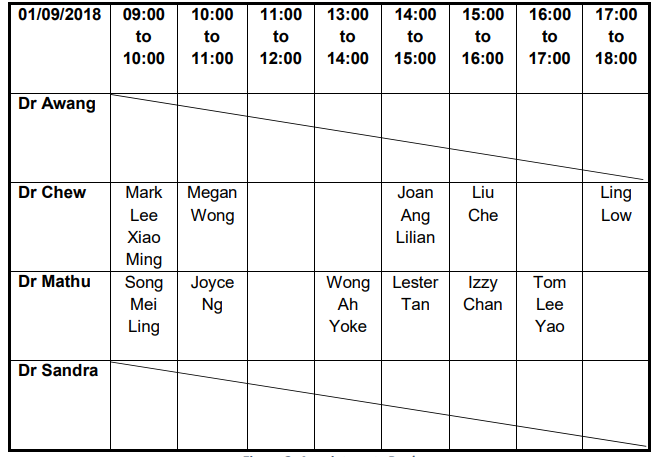
\includegraphics[width=0.5\paperwidth]{C:/Users/Admin/Desktop/Github/question_bank/LyX/static/img/9597-JJC-2018-P2-Q2-1}
\par\end{center}

\noindent \begin{center}
Figure 2: Appointments Book 
\par\end{center}

\noindent\fbox{\begin{minipage}[t]{1\columnwidth - 2\fboxsep - 2\fboxrule}%
Date: 01/09/2018 

Dentist name: Dr Mathu 

09:00: Song Mei Ling 

10:00: Joyce Ng

\dots{} \dots{}

\bigskip{}
%
\end{minipage}}
\noindent \begin{center}
Figure 3: Appointment List
\par\end{center}

\noindent\fbox{\begin{minipage}[t]{1\columnwidth - 2\fboxsep - 2\fboxrule}%
Dentist name: Dr Mathu 

Dentist address: 6 West Coast Drive, Singapore 120006 

Contact number: 98833567%
\end{minipage}}
\noindent \begin{center}
Figure 4: Dentist Record
\par\end{center}
\begin{enumerate}
\item Explain why the patient name and postal code are needed when the receptionist
handles an appointment booking for a patient. \hfill{}{[}2{]}
\item Explain, using two examples, how such a system may compromise data
integrity. \hfill{}{[}4{]}
\item Describe, using an example, how such a system has data redundancy.
\hfill{}{[}2{]}
\item Each patient may book a maximum of one appointment per day. A fully
normalised database solution to this problem is designed. Draw an
E-R diagram that shows these tables and the relationships between
them. \hfill{}{[}4{]}
\item Hence, write the table descriptions. You may introduce additional
attribute(s). Underline the primary keys.\hfill{} {[}3{]}
\item State three fields that require data validation. Suggest a suitable
type of check for each field. \hfill{}{[}3{]}
\end{enumerate}